\documentclass[10pt,twocolumn,a4paper]{article}

\usepackage{amsfonts}
\usepackage{amsmath}
\usepackage{geometry}
\usepackage{xcolor,graphicx}
%\usepackage[subfolder,cleanup]{gnuplottex}
%\usepackage{amsthm}
%\usepackage{enumitem}
%\usepackage{wrapfig}
\usepackage{subcaption}
%\usepackage{hyperref}
\usepackage{tikz}
\usepackage{cite}

\usetikzlibrary{patterns,decorations.pathreplacing}
\usetikzlibrary{arrows.meta}
\usetikzlibrary{shapes.arrows, fadings}

\let\originalleft\left
\let\originalright\right
\renewcommand{\left}{\mathopen{}\mathclose\bgroup\originalleft}
\renewcommand{\right}{\aftergroup\egroup\originalright}

\providecommand{\df}{\textrm{d}}
\newcommand{\diff}[3][\hspace{-0.5pt}]{\frac{\textrm{d}^{#1}#2}{\textrm{d}{#3}^{#1}}}
\newcommand{\pdiff}[3][\hspace{-0.5pt}]{\frac{\partial^{#1}#2}{\partial{#3}^{#1}}}
\newcommand{\Es}{E_{\textrm{sat}}}
\newcommand{\FT}[1]{\mathcal{F}\left\{ #1 \right\}}
\newcommand{\FTi}[1]{\mathcal{F}^{-1}\left\{ #1 \right\}}
\newcommand{\Her}[2]{\widetilde{H}_{#1} \left( #2 \right)}
\DeclareMathOperator{\sech}{sech}
%\newcommand{\eps}{\varepsilon}
%\newcommand{\rect}[1]{\textrm{rect}\left( #1 \right)}

\providecommand{\bigO}[1]{\ensuremath{\mathop{}\mathopen{}\mathcal{O}\mathopen{}\left(#1\right)}}

\newgeometry{margin=1.25cm}

\bibliographystyle{ieeetr}

\title{}
\author{B. Metherall \and C. S. Bohun}

\begin{document}

\twocolumn[
	\begin{@twocolumnfalse}
		\maketitle
		\begin{abstract}

		\end{abstract}
	\end{@twocolumnfalse}
]

\section{Introduction}
\label{sec:intro}
Tuneable lasers have the ability to vary the frequency of its output by up to about 100 nanometres \cite{bohun2015, burgoyne2010, yamashita2009} and simultaneously lase at all frequencies within this bandwidth in short pulses. This tuneability leads to applications such as optical coherence tomography \cite{bohun2015, burgoyne2014, yamashita2009}, coherent anti-Stokes Raman spectroscopy \cite{burgoyne2014}, deep tissue multi-photon microscopy \cite{chung2017, liu2017}, and diagnostics of ultrafast processes \cite{burgoyne2014, silfvast2004}. Tuneable lasers are usually constructed in a ring with five components: an output coupler, chirped fibre Bragg grating (CFBG), modulator, Er-doped fibre, and a pump laser. A typical tuneable ring laser cavity is depicted in Figure \ref{fig:cavity}. Due to the high power and short duration of the pulses, the Kerr nonlinearity becomes crucial to the dynamics within the cavity.

The nonlinearity causes several effects to arise within the laser cavity due to the interplay of dispersion, modulation, and the nonlinearity \cite{bohun2015, coen1997, lapre2019, shao2019, woodward2018}. The two effects of most interest for this paper are optical wave breaking, and modulation instability. Wave breaking causes the leading edge of a pulse to be red shifted, and the trailing edge blue shifted (in the anomalous dispersion regime, the effect is reversed) to the point that a shock is developed \cite{anderson1992, rothenberg1989a, rothenberg1989b, tomlinson1984, tomlinson1985}. The shift in frequencies cause the pulse to become rectangular in the frequency domain with a linear chirp over most of the pulse. In optics, wave breaking manifests from self-phase modulation (SPM) which is a direct effect of the nonlinearity causing the pulse to interfere with itself. This interference generates new frequencies which induces the rectangular profile \cite{agrawal2013, mollenauer1980, woodward2018}. Outside of optics, wave breaking occurs in other areas with nonlinear waves such as plasmas, heat propagation, transmission lines, and fluid dynamics \cite{rothenberg1989b}. Modulation instability is another effect that will be of interest that typically arises in the anomalous dispersion regime. However, in the presence of multiple pulses modulation instability can emerge in the normal dispersion regime as well through cross-phase modulation (XPM) and four-wave mixing (FWM) \cite{agrawal1987, agrawal1989, agrawal2013, haelterman1992}. Modulation instability causes a wave to break into short pulses, and can cause a laser to lose coherence \cite{agrawal1987, coen1997, haelterman1992}. Within a ring laser cavity wave breaking and modulation instability can become parasitic leading to an unstable and unsustainable pulse. This gives rise to the need of understanding the rich landscape of the parameter space, and determining design principles to guarantee the ring laser is stable and sustainable \cite{bohun2015, burgoyneemail, finot2008, lapre2019, woodward2018}.

In Section \ref{sec:modelling}, we briefly review previous mathematical models for the evolution of laser pulses, then we derive our own model in Section \ref{sec:model}. We then examine the results of our model in Section \ref{sec:results}---first solving the model analytically assuming the absence of the nonlinearity, then numerically solving the full nonlinear model. Finally, the concluding thoughts and possible directions of future work are given in Section \ref{sec:conclusion}.

\section{Modelling Efforts}
\label{sec:modelling}
The standard equation for studying nonlinear optics is the nonlinear Schr\"odinger equation (NLSE),
\begin{align}
	\pdiff{A}{z} &= - i \frac{\beta_2}{2}\pdiff[2]{A}{T} + i \gamma |A|^2 A.
	\label{eq:smallnlse}
\end{align}
Here $A = A(T, z) : \mathbb{R}^2 \mapsto \mathbb{C}$ is the complex pulse amplitude, $\beta_2 \in \mathbb{R}$ is the second order dispersion, and $\gamma \in \mathbb{R}$ is the coefficient of nonlinearity. In practice, the NLSE, \eqref{eq:smallnlse}, lacks a few key terms, thus, it is often generalized by adding amplification and loss (occasionally higher order terms are added as well). These additions give the generalized nonlinear Schr\"{o}dinger equation (GNLSE) \cite{agrawal2013, bohun2015, finot2008, peng2018, shtyrina2017, yarutkina2013},
	\begin{align}
	\pdiff{A}{z} &= - i \frac{\beta_2}{2}\pdiff[2]{A}{T} + i \gamma |A|^2 A + \frac{1}{2}g(A) A - \alpha A,
	\label{eq:nlse}
\end{align}
where $g(A)$ is an amplifying term due to the gain, and $\alpha \in \mathbb{R}^+$ is the loss due to scattering and absorption.

\begin{figure}[tbp]
	\centering
	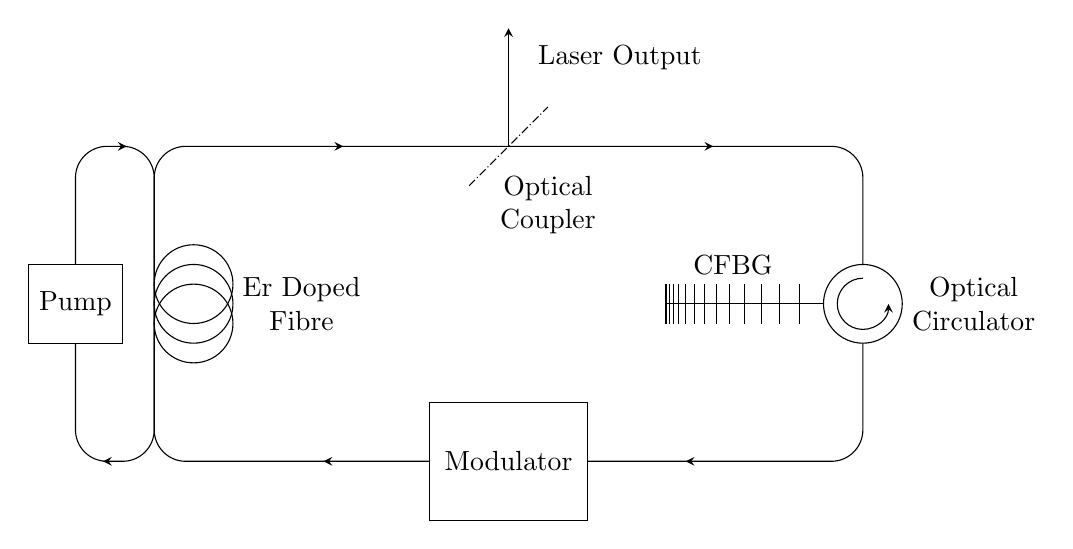
\begin{tikzpicture}
% Two laser loops
\draw [rounded corners=4mm] (0,0) rectangle ++(9,4);
\draw [rounded corners=4mm] (0,0) rectangle ++(-1,4);

% Gain
\draw (0.5,2.25) circle (0.5cm);
\draw (0.5,2) circle (0.5cm) node [anchor=west,xshift=0.5cm,align=center] {Er Doped \\ Fibre};
\draw (0.5,1.75) circle (0.5cm);

% Modulator and pump
\filldraw[fill=white, draw=black] (3.5,-0.75) rectangle ++(2,1.5) node [midway] {Modulator};
\filldraw[fill=white, draw=black] (-1.6,1.5) rectangle ++(1.2,1) node [midway] {Pump};

% Coupler and output
\draw[-stealth] (4.5,4) -- (4.5,5.5) node [pos=0.75,anchor=west,xshift=0.25cm] {Laser Output};
\draw[densely dashdotted] (4,3.5) -- (5,4.5) node [pos=1,anchor=north,yshift=-0.75cm,align=center] {Optical \\ Coupler};

% Circulator
\filldraw[fill=white, draw=black] (9,2) circle (0.5cm) node [anchor=west,xshift=0.5cm,align=center] {Optical \\ Circulator};
\draw[->,>=stealth] (9,2.325) arc (90:360:0.325cm);

% Grating
\draw (8.5,2) -- (6.5,2) node [pos=0.5,anchor=south,yshift=0.25cm,xshift=-0.15cm] {CFBG};
\foreach \i in {0,...,13}
  \draw (6.5 + \i*\i/100,1.75) -- (6.5 + \i*\i/100,2.25);

% Arrows
\draw[-stealth] (2.16,0) -- (2.15,0);
\draw[-stealth] (2.39,4) -- (2.4,4);
\draw[-stealth] (6.76,0) -- (6.75,0);
\draw[-stealth] (7.09,4) -- (7.1,4);
\draw[-stealth] (-0.649,0) -- (-0.65,0);
\draw[-stealth] (-0.351,4) -- (-0.35,4);H
\end{tikzpicture}
	\caption{Typical cavity of a fibre ring tuneable laser \cite{burgoyne2014, chung2017, lapre2019, shao2019, tang2014}. The laser pulses travel clockwise around each loop.}
	\label{fig:cavity}
\end{figure}

The GNLSE has many applications in nonlinear optics and fibre optic communications, however, in laser physics typically a modulation term is also added to ensure mode-locking, this yields the master equation of mode-locking \cite{haus1984, haus1975, haus1986, haus1992, haus2000, tamura1996, usechak2005},
\begin{align}
	\pdiff{A}{z} &= - i \frac{\beta_2}{2}\pdiff[2]{A}{T} + i \gamma |A|^2 A + \frac{1}{2}g(A) A - \alpha A - M(T).
	\label{eq:meml}
\end{align}
No analytic solution is known for \eqref{eq:meml}---even after making the assumptions that the gain is constant, and the modulation is quadratic \cite{haus1984, haus1975, haus1996}. However, by neglecting certain terms of \eqref{eq:meml} analytic solutions can be found \cite{burgoyne2014, haus1975, haus1986, haus1991, haus1992, haus1996, tamura1996, usechak2005}. Furthermore, see Haus \cite{haus2000} for a comprehensive description and history of the theory of mode-locked lasers.

\subsection{Discrete Models}
\label{sec:discrete}
Unfortunately, the master equation, \eqref{eq:meml}, is not completely representative of the underlying physics within our laser cavity. In the derivation of \eqref{eq:meml} it is assumed each process affects the pulse continuously within the cavity. As highlighted by Figure \ref{fig:cavity}, this can be a poor assumption. Within the cavity, each effect is localized to its corresponding component: almost all of the dispersion happens within the CFBG \cite{agrawal2002}, the pulse is only amplified within the Erbium-doped fibre, etc. Thus, a better model is one where we consider a simplified version of the master equation, \eqref{eq:meml}, for each component. Solving these simplified differential equations yields an algebraic expression for the effect of each individual component. The relations can then be functionally composed to give an iterative map for the effect of one round trip of the cavity.

Such a method was first proposed in 1955 by Cutler \cite{cutler1955} while analyzing a microwave regenerative pulse generator. This method was adapted for mode-locked lasers in 1969 by Siegman and Kuizenga \cite{kuizenga1970a, kuizenga1970b, kuizenga1970, siegman1969}. The effects of the nonlinearity would not be considered until Martinez, Fork, and Gordon \cite{martinez1984, martinez1985} tried modelling passively mode-locked lasers. This issue has recently been readdressed by Burgoyne \cite{burgoyne2014} in the literature for tuneable lasers. In each of these models the effect of each block is described by a transfer function.

Despite the development of these block style models, several short-comings exist. The clearest is that none of these models have contained every block---either the nonlinearity or the modulation have been omitted. Each component of a tuneable plays a crucial role and the laser will not function correctly without the inclusion of all of the components. Another drawback is that the functional operations of some of the components used in their models are phenomenological. While these functions are chosen based on the observed output, they are not necessarily consistent with the underlying physics. Finally, none of these previous models have been able to fully exhibit the instabilities described in Section \ref{sec:intro}.

\section{Model Derivation}
\label{sec:model}
Using the idea of a discrete model presented Section \ref{sec:discrete}, we derive our model from the GNLSE, \eqref{eq:nlse}; however, in the case of the modulation we consider the exact functional form to be determined by the laser operator. To accomplish this we follow the method described in Section \ref{sec:discrete}; we neglect all terms but one on the right side of \eqref{eq:nlse} and solve the simplified differential equations.

To proceed we must choose the form of the amplification term, $g(A)$. We assume the gain has the form
\begin{align}
	g(A) &= \frac{g_0}{1 + E / \Es},& E &= \int_{-\infty}^\infty |A|^2 \, \df T,
	\label{eq:energy}
\end{align}
where $g_0$ is a small signal gain, $E$ is the energy of the pulse, and $\Es$ is the energy at which the gain begins to saturate \cite{haus1984, shtyrina2017, silfvast2004}. This reduces the GNLSE, \eqref{eq:nlse}, to
\begin{align}
	\pdiff{A}{z} &= \frac{g_0 A}{2 \left( 1 + E / \Es \right)}.
\end{align}
By assuming $E(0) = E$ and $E(L_g) = E_{\text{out}}$, we find the energy after amplification is
\begin{align}
	\label{eq:engain}
	E_{\text{out}} &= \Es W \left( \frac{E}{\Es} \textrm{e}^{E / \Es} \textrm{e}^{g_9 L_g} \right),
\end{align}
where $W$ is the Lambert $W$ function \cite{corless1996}. Rewriting \eqref{eq:engain} in terms of the pulse gives
\begin{align}
	G(A) &= \left( \frac{\Es}{E} W \left( \frac{E}{\Es} \textrm{e}^{E/\Es} \textrm{e}^{g_0 L_g} \right) \right)^{1/2} A
\end{align}
for the amplification of the pulse within the Er-doped fibre. Repeating this process for the loss, dispersion, and nonlinearity yields
\begin{align}
	L(A) &= (1 - R) \textrm{e}^{- \alpha L_T}A, \\
	D(A) &= \FTi{\textrm{e}^{i \omega^2 L_D\beta_2/2} \FT{A}}, \\
	F(A) &= A \textrm{e}^{i \gamma |A|^2 L_f},
\end{align}
where $R$ is the reflectivity of the output coupler (depending on the layout of the laser cavity the loss may instead take the form $L(A) = R \textrm{e}^{- \alpha L_T}A$), $L_T$ is the total length of the laser circuit, $L_D$ is the length of the dispersive medium, $L_f$ is the length of fibre between the amplifier and the output coupler, and where $\mathcal{F}$ denotes the Fourier transform. Finally, we must assume a form for the modulation. The modulation is considered to be applied externally in which ever way the operator sees fit. For simplicity the representation is taken as the Gaussian
\begin{align}
	M(A) &= \textrm{e}^{-T^2 / 2 T_M^2} A,
	\label{eq:modform}
\end{align}
where $T_M$ is the characteristic width of the modulation. This assumption is not particularly restrictive. Calcaterra and Boldt have shown that Gaussians can form a basis for $L^2(\mathbb{R})$ \cite{calcaterra2008a}. Therefore, we can approximate any modulation function in $L^2(\mathbb{R})$ by a sum of \eqref{eq:modform}.

\subsection{Non-Dimensionalization}
The structure of each process of the laser can be better understood by re-scaling the time, energy, and amplitude; this suggests the convenient scalings:
\begin{align}
	T &= T_M \widetilde{T},& E &= \Es \widetilde{E},& A &= \left( \frac{\Es}{T_M} \right)^{1/2} \widetilde{A}.
\end{align}
Revisiting each process map shows each process has a characteristic non-dimensional parameter. The new mappings---after dropping the tildes---are
\begin{equation}
	\begin{aligned}
		G(A) &= \left(E^{-1} W \left( a E \textrm{e}^{E}\right) \right)^{1/2} A, & F(A) &= A \textrm{e}^{i b |A|^2}, \\
		D(A) &= \FTi{\textrm{e}^{i s^2 \omega^2} \FT{A}}, & L(A) &= h A, \\
		M(A) &= \textrm{e}^{-T^2 / 2} A,
		\label{eq:effects}
	\end{aligned}
\end{equation}
with the four dimensionless parameters,
\begin{equation}
	\begin{aligned}
		a &= \textrm{e}^{g_0 L_g} \sim 8 \times 10^3,& \qquad h &= (1 - R) \textrm{e}^{-\alpha L} \sim 0.04, \\
		b &= \gamma L_f \frac{\Es}{T_M} \sim 1,& \qquad s &= \sqrt{\frac{\beta_2 L_D}{2 T_M^2}} \sim 0.2,
		\label{eq:ndparam}
	\end{aligned}
\end{equation}
which characterize the behaviour of the laser. Nominal values for the parameters, \eqref{eq:ndparam}, can be found in \cite{agrawal2002, agrawal2013, bohun2015, burgoyne2014, burgoyneemail, finot2008, li1998, litchinitser1997, peng2018, shtyrina2017, tamura1993, tamura1996, tomlinson1984, usechak2005, yamashita2009, yarutkina2013}. Notice that the modulation is only characterized by $T_M$, and each other process has its own associated independent non-dimensional parameter.

% Table of parameter values
% \begin{table*}[tbp]
% 	\centering
% 	\begin{tabular}{lcll}
% 		\hline\noalign{\smallskip}
% 		Parameter & Symbol & Value & Sources \\
% 		\hline\noalign{\smallskip}
% 		Absorption of Fibre & $\alpha$ & $10^{-4}$--$0.3\text{ m}^{-1}$  & \cite{burgoyneemail, shtyrina, tomlinson, usechak, yarutkina} \\
% 		Fibre Dispersion & $\beta_2^f$ & $-50$--$50 \text{ ps}^2/ \text{km}$ & \cite{agrawal2002, agrawal2013, burgoyne2014, litchinitser, peng, yarutkina} \\
% 		Fibre Nonlinearity & $\gamma$ & $0.001$--$0.01 \text{ W}^{-1} \text{m}^{-1}$ & \cite{agrawal2013, finot, usechak, yarutkina} \\
% 		Grating Dispersion & $\beta_2^g L_D$ & $10$--$2000 \text{ ps}^2$ & \cite{agrawal2002, agrawal2013, burgoyne2014, li} \\
% 		Length of Cavity & $L_T$ & $10$--$100 \text{ m}$ & \cite{burgoyneemail, peng, tamura1996} \\
% 		Length of Fibre & $L_f$ & $0.15$--$1 \text{ m}$ & \cite{burgoyneemail} \\
% 		Length of Gain Fibre & $L_g$ & $2$--$3 \text{ m}$ & \cite{burgoyne2014, peng, shtyrina, tamura1993, yarutkina} \\
% 		Modulation Time & $T_M$ & $15$--$150 \text{ ps}$ & \cite{bohun, burgoyneemail, burgoyne2014} \\
% 		Reflectivity of Optical Coupler & $R$ & $0.1$--$0.9$ & \cite{burgoyneemail, li, peng,  tamura1993, tamura1996, yamashita} \\
% 		Saturation Energy & $\Es$ & $10^3$--$10^4 \text{ pJ}$ & \cite{burgoyneemail, usechak, yarutkina} \\
% 		Small Signal Gain & $g_0$ & $1$--$10 \text{ m}^{-1}$ & \cite{burgoyneemail, yarutkina} \\
% 		\noalign{\smallskip}\hline
% 	\end{tabular}
% 	\caption{Range of variation of various parameters.}
% 	\label{tab:values}
% \end{table*}

\subsection{Combining the Effects}
\label{sec:effects}

\begin{figure}[tbp]
	\centering
	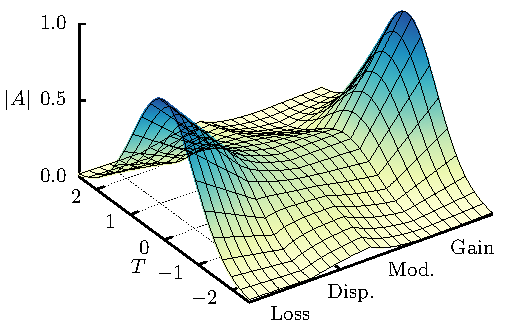
\includegraphics{Evo}
	\caption{Evolution of the envelope during one round trip of the cavity at equilibrium. The pulse decays due to the output coupler, dispersed by the CFBG, modulated by the modulator, and finally amplified by the gain fibre (the envelope is unaltered by the nonlinearity). Note that this is for visualization only, the durations are not to scale.}
	\label{fig:cavityevo}
\end{figure}

Now that we have the algebraic effect of each section of the cavity, we are ready to compose each map together to give the effect of one round trip of the cavity. Thus, we must now consider the order of the components. As we are most interested in the output of the laser cavity, we shall start with the loss. We then pass the pulse through the CFBG followed by the modulator. The pulse then travels through the Er-doped fibre to be amplified, and finally we consider the effect of the nonlinearity. The nonlinearity must immediately follow the gain---this is the section of the cavity where the pulse is most energetic, and hence, has the largest effect. Note, the permutation of the other components is indeed important as the operators do not, in general, commute---this is in contrast to the models described in Section \ref{sec:discrete}. Moreover, we prefer the loss to follow the gain and nonlinearity as we wish to minimize the length over which the nonlinearity has an effect, and maximize the output power. Functionally we denote one round trip of the cavity by
\begin{align}
	\mathcal{L}(A) = F(G(M(D(L(A))))).
	\label{eq:order}
\end{align}
 The pulse after one complete circuit of the laser cavity is then returned back into the cavity to restart the process. A steady solution to this model is one in which the envelope and chirp are unchanged after traversing every component in the cavity---we are uninterested in the phase. That is, such that $\mathcal{L}(A) = A \textrm{e}^{i \phi}$---for some $\phi \in \mathbb{R}$. An example of the evolution of the envelope during one round trip of the laser cavity can be found in Figure \ref{fig:cavityevo}.

\section{Results}
\label{sec:results}
We split the results into two subsections. In the following subsection we investigate the low nonlinearity limit, and in Section \ref{sec:nlresults} we look at the full nonlinear model.

\subsection{Linear Solution}
By neglecting the effect of the nonlinearity, that is, $b = 0$, a solution can be found analytically. We assume the solution will take the form of a chirped Gaussian. There are a few reasons for this; the solution to the models presented in \cite{cutler1955, siegman1969, kuizenga1970a, martinez1984, martinez1985} were Gaussian, the equilibrium shape will be highly correlated to the shape of the modulation function, and since a Gaussian is a fixed point of the Fourier transform \cite{gradshteyn2007}. Furthermore, this form is chosen because it resembles the envelope and linear chirp expected \cite{burgoyne2014, haus1975, haus1996, haus2000, usechak2005}.

To compute $\mathcal{L}(A)$, consider the pulse
\begin{align}
	A = \sqrt{P} \exp \left( -(1 + iC) \frac{T^2}{2 \sigma^2} \right) \textrm{e}^{i \phi_0},
	\label{eq:A0}
\end{align}
where $P$ is the peak power, $C$ is the chirp, $\sigma^2$ is the variance, and $\phi_0$ is the initial phase. This pulse shape is depicted in Figure \ref{fig:samplegauss}.

\begin{figure}[tbp]
	\centering
	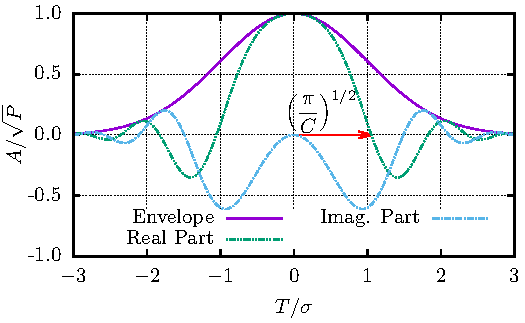
\includegraphics{Sample_Gauss}
	\caption{Solution to the linear model given by \eqref{eq:A0}.}
	\label{fig:samplegauss}
\end{figure}

To compute $\mathcal{F}(A)$, given the initial pulse \eqref{eq:A0}, we iteratively compute the effect of each process map from \eqref{eq:effects}. Now, by equating $\mathcal{F}(A)$ and $A \textrm{e}^{i \phi}$ we obtain a system of equations. In particular,
\begin{gather}
	\sigma^8 + 4 s^4 \sigma^6 - 20 s^4 \sigma^4 + 32 s^4 \sigma^2 - 16 s^4 = 0, \label{eq:var} \\
	C = \frac{\sigma^4 \pm \sqrt{\sigma^8 - 16 s^4 \left( 1 - \sigma^2 \right)^2}}{4 s^2 \left( 1 - \sigma^2 \right)}.
	\label{eq:chirp}
\end{gather}

As \eqref{eq:var} is a quartic in $\sigma^2$ it has an analytic solution, namely,
\begin{equation}
	\begin{split}
		\sigma^2 = \sqrt{2} s \left( s^6 + 3s^2 + \sqrt{4 + s^4} \left( 1 + s^4 \right) \right)^{1/2} & \\
		- s^4 - s^2 & \sqrt{4 + s^4},
		\label{eq:equilvar}
	\end{split}
\end{equation}
which can readily be used to find the chirp, $C$. By asymptotically expanding \eqref{eq:var} we find the useful relations
\begin{align}
	\sigma^2 &\sim
	\begin{cases}
		2s(1 - s) + \bigO{s^3} & s \rightarrow 0 \\
		1 - \frac{1}{4}s^{-4} + \frac{3}{8}s^{-8} + \bigO{s^{-12}} & s \rightarrow \infty,
	\end{cases} \\
	C &\sim
	\begin{cases}
		1 - s + \frac{1}{2}s^2 + \bigO{s^3} & s \rightarrow 0 \\
		\frac{1}{2}s^{-2} - \frac{3}{8}s^{-6} + \bigO{s^{-10}} & s \rightarrow \infty.
	\end{cases}
\end{align}
The equilibrium energy and peak power can be found by conservation of energy to give
\begin{align}
	E = \frac{h^2 \left( 1 - \sigma^2 \right)^{1/2}}{1 - h^2 \left( 1 - \sigma^2 \right)^{1/2}} \log \left( a h^2 \left( 1 - \sigma^2 \right)^{1/2} \right),
\end{align}
and
\begin{align}
	P = \frac{W(a E \textrm{e}^E)}{\sqrt{\pi} \sigma},
	\label{eq:equilpower}
\end{align}
respectively.

Our linearized model indeed exhibits the same form as previous linear models. However, by including the effects of the nonlinearity we uncover the rich interplay between dispersion, modulation, and nonlinearity not previously found mathematically.

\subsection{Nonlinear Solution and Instability}
\label{sec:nlresults}
In this iterative scheme---as well as within the laboratory---we must specify the input pulse shape. The most common form is a hyperbolic secant \cite{coen1997, finot2008, mitschke1986, rothenberg1989b, tomlinson1984}, which we assume has the exact form
\begin{align}
	A_0 = \Gamma \sech \left( 2 T \right) \textrm{e}^{i \pi / 4},
	\label{eq:nlA0}
\end{align}
where $\Gamma$ is a normalizing factor chosen so the pulse has an initial energy of $E_0 = 0.1$, unless specified otherwise.

\begin{figure}[tbp]
	\centering
	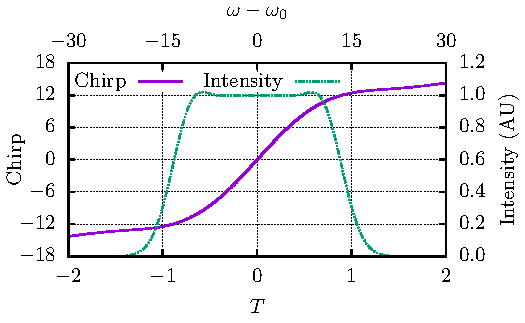
\includegraphics{ChirpFT}
	\caption{Chirp and Fourier transform in equilibrium state obtained by \eqref{eq:nlA0}, with values $a = 8 \times 10^3$, $h = 0.04$, $b = 1$, $s = 0.2$, and $E_0 = 0.1$.}
	\label{fig:chirpft}
\end{figure}

In Figure \ref{fig:chirpft} we show the chirp and Fourier transform of the pulse \eqref{eq:nlA0} once it has reached equilibrium for the nominal parameter values given in \eqref{eq:ndparam}. In this nonlinear case, we find that the equilibrium pulse is no longer Gaussian---as evidenced by the Fourier transform. Notice that compared to the linear case, higher frequency modes are introduced due to the nonlinearity. Moreover, we find the pulse is linearly chirped near the peak, but, in the tails, $|T| > 1$, the chirp begins to saturate---consistent with experimental results \cite{chen2008, rothenberg1989b, tomlinson1985}. As the nonlinearity parameter, $b$, is increased, the two lobes in the Fourier transform become more pronounced. However, once a critical point is reached SPM begins to play a more substantial factor, leading to modulation instability. This phenomenon is highlighted in Figure \ref{fig:breakevo}. By increasing the nonlinearity, and decreasing the dispersion we find the pulse begins to `breathe'. During the first two dozen round trips of the cavity, the SPM compounds and becomes too parasitic to the pulse. This in turn induces modulation instability, and degrades the pulse, making the pulse no longer stable or sustainable. On the other hand, having a more moderate value of $b$, the pulse is able to equilibrate even with a less favourable initial pulse (Figure \ref{fig:convevo}). The pulse is able to shed the initial left lobe because of dispersion and modulation, and the central lobe is able to grow due to the gain medium. This allows the pulse to come to equilibrium very quickly. Furthermore, since the intensity of the initial pulse is relatively small, the effect of SPM is negligible during the first few round trips which allows the laser to select preferable modes. These preferable modes then get amplified which stabilizes the pulse. From this, it is clear the initial shape of the pulse is much less important than the initial energy of the pulse, $E_0$, or the strength of the nonlinearity, $b$.

\begin{figure}[tbp]
	\centering
	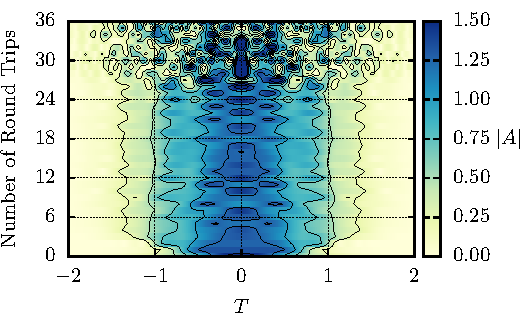
\includegraphics{Break}
	\caption{Example of a pulse destabilizing from the initial pulse \eqref{eq:nlA0} ($a = 8 \times 10^3$, $h = 0.04$, $b = 1.6$, $s = 0.1$, and $E_0 = 0.1$).}
	\label{fig:breakevo}
\end{figure}

\begin{figure}[tbp]
	\centering
	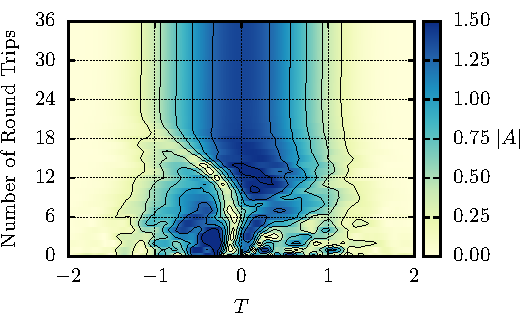
\includegraphics{Conv}
	\caption{Example of a pulse coming to equilibrium from noise ($a = 8 \times 10^3$, $h = 0.04$, $b = 1.0$, $s = 0.1$, and $E_0 = 0.1$).}
	\label{fig:convevo}
\end{figure}

We now turn our attention to characterizing the stability of a laser by exploring the parameter space. We focus on the $s$--$b$ plane in particular since $a$ and $h$ effect only the amplitude of the pulse and do not contribute to the interplay of dispersion and the nonlinearity. Additionally, a conservative initial energy will effect the dynamics much less than a more intense pulse since the nonlinearity will be negligible while coming to equilibrium. To identify the stability of a pulse we examine the relative change in the pulse's envelope between consecutive iterations. We compute this error by
\begin{align}
	\textrm{E} = \frac{\| |A_i| - |A_{i-1}| \|_2}{\| A_{i-1} \|_2},
	\label{eq:error}
\end{align}
where $\| \cdot \|_2$ denotes the $L^2(\mathbb{R})$ norm, and $i$ is chosen to be sufficiently large to guarantee the pulse reaches equilibrium or degrades due to modulation instability---we use $i = 250$ in our experiments (Figure \ref{fig:error}). Note that we take the modulus of the pulse since we are only interested in the evolution of the envelope. We find a very sharp and rich boundary between two regions. In the upper-left region the error is $\bigO{1}$, this is where the nonlinearity is too strong, and the SPM induces modulation instability. In the lower-right region we find the opposite behaviour---the pulse reaches an equilibrium state and is stable. The error is on the order of machine precision, or slightly higher due to approximating a smooth continuous function by discrete points.

\begin{figure}[tbp]
	\centering
	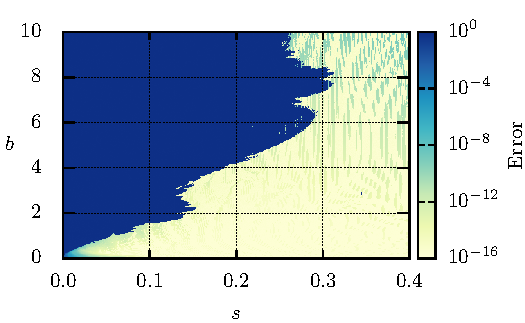
\includegraphics{ParamSpaceErr}
	\caption{Relative error of a pulse's envelope between round trips 249 and 250 ($a = 8 \times 10^3$, $h = 0.04$, and $E_0 = 0.1$).}
	\label{fig:error}
\end{figure}

Also of interest is the energy of the pulse at equilibrium. We compute the energy using \eqref{eq:energy}, or equivalently 
\begin{align}
	E &= \| A_i \|_2,
	\label{eq:energy2norm}
\end{align}
where, again, $i = 250$ in our experiments. Recall from \eqref{eq:order}, this energy is the immediately before passing through the output coupler, and so the energy of each pulse emitted by the laser is instead $(1 - h^2) \| A_i \|_2$, and $h^2 \| A_i \|_2$ remains in the cavity. We plot \eqref{eq:energy2norm} in Figure \ref{fig:energy}. Unsurprisingly, we find the same sharp boundary as we saw in Figure \ref{fig:error}. In the unstable region (upper-left) the energy is relatively small. Since the pulse is not stable in this region it is not able to foster prominent modes, thus, the intensity is low across the entire pulse. In the stable region (lower-right) we find that the energy smoothly decays as both $b$ and $s$ increase, with the contours being hyperbolic-esque. From this it is clear that a more energetic laser requires weaker dispersion, however, the nonlinearity must be correspondingly low, otherwise modulation instability will destroy the pulse.

\begin{figure}[tbp]
	\centering
	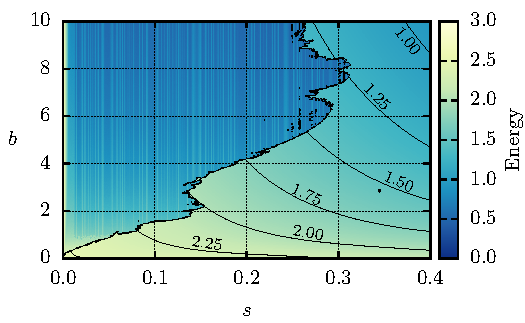
\includegraphics{ParamSpaceEnergy}
	\caption{Energy of the pulse after 250 round trips ($a = 8 \times 10^3$, $h = 0.04$, and $E_0 = 0.1$).}
	\label{fig:energy}
\end{figure}

Finally, we briefly look at how the order of the components effects the dynamics. In Section \ref{sec:effects} we justified the order of the gain, nonlinearity, and loss, but, just assumed dispersion preceded modulation. Here we consider the effect of swapping the dispersion and modulation components. The energy landscape (Figure \ref{fig:energyswitch}) is as we would expect. In the previous case of having modulation following dispersion, more energy is removed from the pulse tails. Whereas, having modulation first, more of this energy remains in the cavity. This has the effect of making the laser more powerful, which in turn increases the unstable region. Comparing with Figure \ref{fig:energy}, this is what we find. The unstable upper-left region spreads farther rightward, and the energy is larger in the stable region---especially farther away from the origin.

\begin{figure}[tbp]
	\centering
	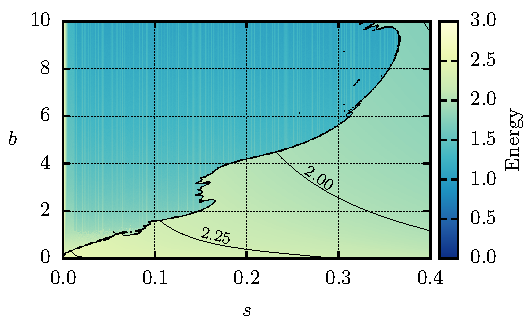
\includegraphics{ParamSpaceEnergySwitch}
	\caption{Energy of the pulse after 250 round trips with dispersion and modulation swapped ($a = 8 \times 10^3$, $h = 0.04$, and $E_0 = 0.1$).}
	\label{fig:energyswitch}
\end{figure}

\section{Conclusion}
\label{sec:conclusion}
Expanding upon the ideas originally proposed by Cutler \cite{cutler1955}, and Kuizenga and Siegman \cite{kuizenga1970, kuizenga1970a, siegman1969}, we developed a nonlinear functional model for tuneable ring lasers. We recover linearly chirped Gaussian solutions in the case of a Gaussian modulation function when omitting the nonlinearity. Moreover, the solution of the linear model can easily be extended to any modulation function using results of \cite{calcaterra2008a}. In contrast, with the inclusion of the nonlinearity we were able to recover wave breaking and modulation instability, and found a sharp boundary of stability. This phenomenon has been demonstrated in a laboratory setting \cite{agrawal2013, anderson1992, finot2008, rothenberg1989b, tomlinson1985}, but, has difficult to predict with mathematical models. Furthermore, it is of interest to analyze the nonlinear model analytically using an asymptotic expansion for small values of the nonlinearity parameter, $b$. Doing so would provide insight to how the nonlinearity impacts the linearized solution to better understand the manifestation of wave breaking and modulation instability.

\section*{Acknowledgement.}
BM acknowledges the support provided by the EPSRC Centre for Doctoral Training in Industrially Focused Mathematical Modelling (EP/L015803/1).

\section*{Disclosures.}
The authors declare no conflicts of interest.

\bibliography{Ref}

\end{document}
